\documentclass[letterpaper, 10 pt, conference]{ieeeconf}  % Comment this line out if you need a4paper

%\documentclass[a4paper, 10pt, conference]{ieeeconf}      % Use this line for a4 paper

\IEEEoverridecommandlockouts                              % This command is only needed if 

\overrideIEEEmargins                                     

% The following packages can be found on http:\\www.ctan.org
%\usepackage{graphics} % for pdf, bitmapped graphics files
%\usepackage{epsfig} % for postscript graphics files
%\usepackage{mathptmx} % assumes new font selection scheme installed
%\usepackage{times} % assumes new font selection scheme installed
%\usepackage{amsmath} % assumes amsmath package installed
%\usepackage{amssymb}  % assumes amsmath package installed
\usepackage{graphicx}
\usepackage{verbatim}
\usepackage{amsmath,amssymb}
\usepackage{color} % added by Shani
\newcommand{\argmin}{\arg\!\min}
\newcommand{\argmax}{\arg\!\!\max}
\newtheorem{thm}{Hypothesis}
\linespread{0.968}
\title{\LARGE \bf
Markov Games with Time-variant Types as a Framework for Human-robot Coordination
}
\author{Shih-Yun Lo$^{1}$, Shani Alkoby$^{2}$, Benito Fernandez$^{1}$, and Peter Stone$^{2}$% <-this % stops a space
%\thanks{*This work was supported by }% <-this % stops a space
%\thanks{$^{1}$ Mechanical Engineering Department, the University of Texas at 
%Austin, USA. 
%        University of Twente, 7500 AE Enschede, The Netherlands
%{\tt\small $\{$yunl,benito$\}$@utexas.edu}}
%\thanks{$^{2}$Bernard D. Researcheris with the Department of Electrical Engineering, Wright State University,
%        Dayton, OH 45435, USA
%        {\tt\small b.d.researcher@ieee.org}}%
}

\begin{document}
\maketitle
\thispagestyle{empty}
\pagestyle{empty}
%%%%%%%%%%%%%%%%%%%%%%%%%%%%%%%%%%%%%%%%%%%%%%%%%%%%%%%%%%%%%%%%%%%%%%%%%%%%%%%%
\begin{abstract}
	Coordination between humans and robots commonly happens when they 
	co-exist in a shared workspace. Such scenario includes human-robot teaming on 
	collaborative tasks, and 
	human-robot conflict-resolving on limited shared resources. Mis-coordination 
	reduces 
	efficiency of both parties, and reduces the human's trust and patience with 
	the robot. In this work, we propose a game-theoretic framework to analyze 
	convergence in 
	human-robot coordination.
	We also propose human behavior hypotheses on their 
	decision-making mechanisms under this framework, 
	to capture how the human 1) perception of the robot's capabilities, 2) personal preferences, 3) level of self-interest, and 4) social 
	trust affect their policies and adaptability in dynamic environments. 
	We provide human-robot path crossing as an instantiation of our framework, and use the 
	hypothesized human behaviors to simulate real-world observed interaction 
	patterns. Lastly, we simulate humans acting adaptively to their observed robot 
	policies, as an initiative to incorporate effects on humans when designing 
	robot algorithms using human-human interaction data.
\end{abstract}
\vspace{-.3em}
\section{Introduction}
\vspace{-.2em}
Human-robot interaction has received increased attention in recent years due to the 
emerging interest in deploying robots in human environments. Such 
environments may involve human-robot collaboration on given tasks, 
humans and robots working in a shared workspace, or service 
robots deployed in human environments. In such environments, robots 
may need to coordinate with humans with partially shared information and 
partially shared objectives; agents may need to reach agreement on one 
solution among multiple feasible choices, which makes the coordination non-trivial to 
settle. For a motivating example, see Fig.~\ref{fig:intro}, which shows three agents coordinating at an 
intersection, where each agent has an individual goal to reach. 

For a robot to engage coordination without confusing the human, it first 
requires the basic capabilities to understand human intent, and to respond in a 
legible manner~\cite{dragan2013legibility}. Beyond those, to negotiate and agree on the coordinating 
solutions, the robot needs knowledge of human agents' behaviors to 
predict the outcome of its own actions. 
It also needs to known the reaction time humans need 
to update their policies~\cite{shah2011improved}, and to consider potential 
impacts of its own actions on humans' future 
decisions~\cite{fujiwara2015non,foerster2017learning}. Then the 
robot can plan and coordinate with humans in an intent-consistent fashion. 

Past research has sought to improve human-robot coordination in a variety of 
ways, including: intent-expressive robot 
motion generation~\cite{dragan2013legibility,lichtenthaler2012influence}, human 
preference-aware behavior modeling and its 
use for coordination~\cite{gombolay2015coordination,dorsa2017active}, human-robot mutual 
adaptation~\cite{nikolaidis2013human,nikolaidis2016formalizing}, human 
expectations on robot capability~\cite{cha2015perceived,kwon2016human}, as well as trust and comfort for long-term 
deployment\cite{yang2017evaluating}. 

While these topics share a focus on factors which affect human behaviors and 
their decision-making mechanisms, 
they lack a unifying framework to keep track of how those factors correlate with 
each other in different situations, how they affect human 
decisions and motions, and 
how they evolve over time as a function of robot interaction policies. 
Those questions are important for designing intent-consistent robots to 
interact with humans in daily situations. And they are important for 
designing 
robots that are aware of human 
adaptation to their long-term deployments.  
\begin{figure}[t]
	\centering
	\vspace{-1em}
	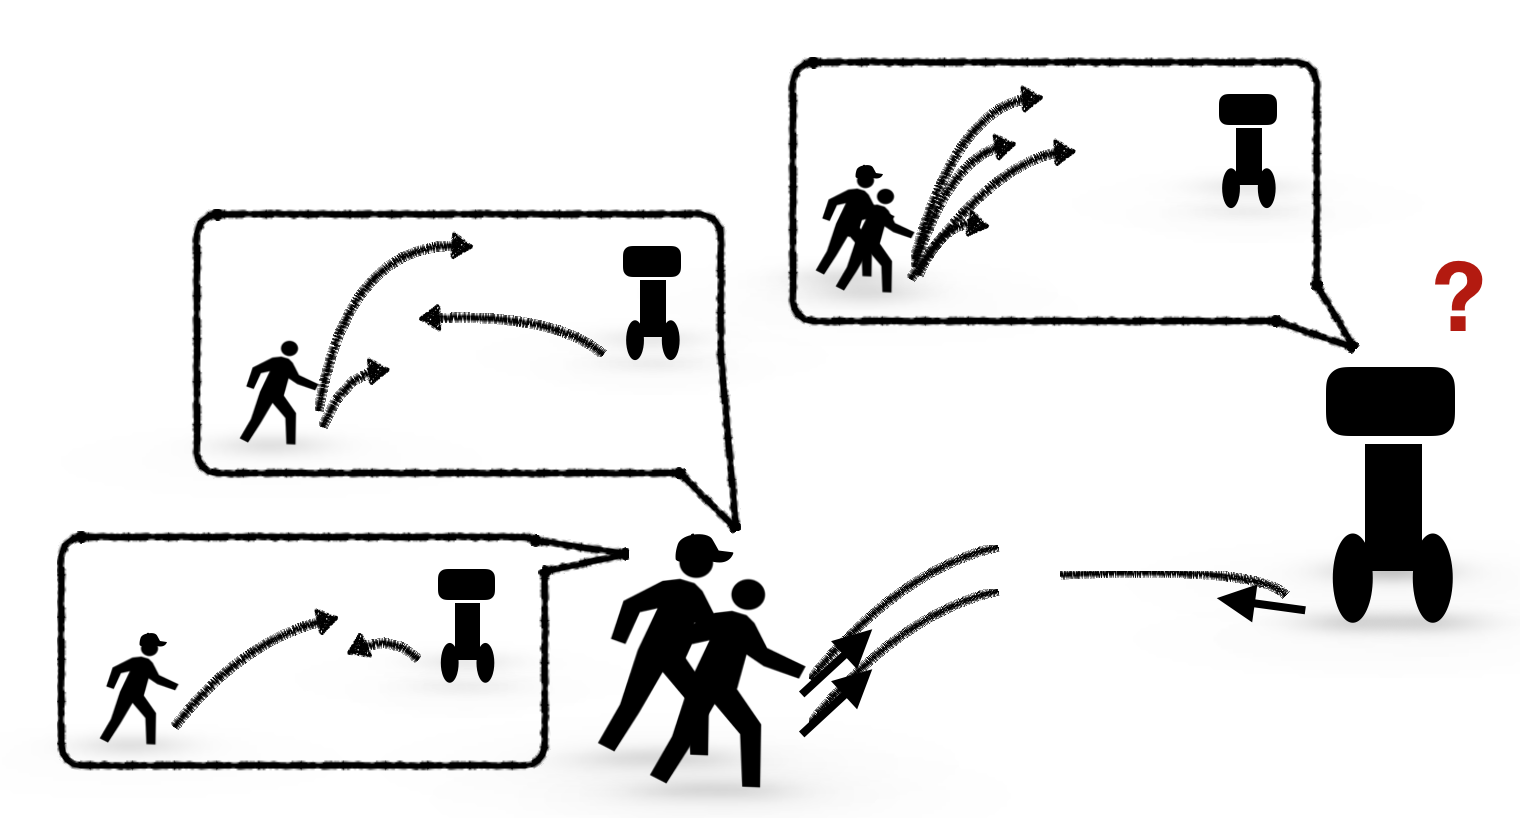
\includegraphics[scale=0.32]{intro}
	\vspace{-1.5em}
	%\hspace{-5em}
	\caption{Human-robot coordination in a crossing interaction. Since 
		people have different prior assumptions on robot behaviors, their choice 
		of actions differ.}
	\vspace{-2em}
	\label{fig:intro}
\end{figure}
To fulfill such purposes, the main contribution of this work is a proposed game-theoretic 
model for human-robot coordination where agents have hidden preferences and time-variant adaptive behaviors based 
on online observations of others' behaviors.

To discuss human behaviors while interacting with robots, we point out some
important factors that have been proposed in the human-robot interaction 
community, such as perceived robot capability, personal preferences, and 
trust on robot ability. We illustrate how they affect human behaviors through 
our proposed human decision-making model under the game framework, using a 
receding-horizon approach. We also propose two factors that we observed to be 
important in the social navigation 
domain: level of self-interest and social trust. We incorporate them along 
with others to analyze how people interact with the robot, with different 
personal preferences and assumptions about robot 
behaviors. We collect real-world human-robot interaction data to 
illustrate our model effectiveness. 

We also use our decision-making model to discuss human adaptability to robots,
and simulate human adaptation to robots after perceiving robot 
socially trust-worthy behaviors. 

\section{Related Work}
Despite the growing interest in deploying robots in human populated workspaces, 
motion planning algorithms for smooth human-robot coordination have remained a 
challenge. While traditional planning algorithms have shown success in static 
environments, deploying such approaches alongside humans has shown 
insufficient adaptability to highly dynamic environments, and produce awkward 
motions making 
interpretability difficult
~\cite{lichtenthaler2012influence,dragan2013legibility,kruse2012legible}. 
Approaches considering time-variant factors, such as temporal constraints for multi-agent collision 
avoidance~\cite{van2011reciprocal}, have drawn attention for such 
applications; approaches considering human factors, such as human 
collision-avoidance behavior anticipation~\cite{helbing1995social}, have also gained attention for robot planning in human workspaces~\cite{shiomi2014towards}.

On the other hand, another community solves robot planning in human environments as a 
joint multi-agent planning problem, to incorporate the collective crowd 
behaviors with explicit modeling of the effect of agent actions on its 
surround agents~\cite{trautman2010unfreezing,kuderer2012feature,mavrogiannis2016decentralized}. Such joint modeling methodology has 
shown to be effective at outputting smooth human-mimicking trajectories at the same 
time acting responsively to its surrounding agents.

One major drawback applying these approaches interacting with humans is that the 
multi-agent joint dynamics models are typically learnt from data collected by 
human demonstrations, whereas humans do not act the same way around a robot compared to in 
pure-human environments. This problem has shown 
inefficiency of such approaches when humans use unexpected behaviors 
around robots -- behaviors that humans will not present in front of another 
human~\cite{pfeiffer2016predicting}. 

To model joint behaviors among agents -- how one's action affects the other -- another way is to incorporate individual's action values with correlations 
with other agents' actions. Such joint behavior formulation is widely studied 
in Game theory: with different player assumptions, games evolve with different 
outcomes. In the artificial intelligence community, such game 
formulation has been incorporated with Markov Decision Process for multi-agent 
reinforcement learning~\cite{littman1994markov}. Such incorporation enables strategy 
design for multi-agent robotic systems with mutual learning. 

Yet, to simulate human-robot interaction, it requires agents modeled after 
humans, who have distinctive learning mechanisms and decision-making processes 
from reinforcement learning agents; moreover, agents have different behavioral 
types, as humans have personal preferences; agents online adapt to other 
agents, as humans observe the others and plan accordingly. Those features are 
widely studied in the human-robot interaction community, but not yet well 
formulated by one unifying framework. We therefore propose 
an extensive framework on Markov games with time-variant types to incorporate 
human-robot interaction with multi-agent learning problems to eliminate the gap. 



\section{Preliminaries}
In almost every real-life interaction between robots and humans, each agent's utility is being influenced by the other agents' actions in addition to his own action. Thus, we choose to model human-robot interaction as a game. We propose a model, extended from Markov Games, to incorporate types as in Bayesian games, which assign game outcomes based on both agent actions and types \footnote{The model can also take in continuous-space input space $U$ to apply to real-world robotics domains}. A formal game definition as well as a quick overview about Markov Games are given in the following subsections.  
\subsection{Game Definition}
Consider a game $G$ with $k$ players, where each player $i \in \{1...k\}$ has 
a finite action set $A^i$. The set of action profiles is denoted as 
$\Sigma = A^1 \times A^2 \times ... \times A^k$. The utility of an 
agent $i$ is a function, denoted as $f^i: \sigma \rightarrow \mathbb{R} $, 
evaluated at $\sigma \in \Sigma$. 

%repeated games
In \textit{repeated games} (i.e., games which repeat for more than one action per player), $G^T$, players receive cumulative utilities over a 
time horizon $T$, defined as:
\begin{equation}
	V^i=\Sigma_{t=0}^{T} f^i_t(\sigma_t).
\end{equation}
Where $\sigma_t$ is the action profile at time $t$.
We will define a \textit{strategy profile} to be the series of action profiles $\sigma_t$ over time, i.e., $s = \sigma_0 \times \cdots \sigma_T \in S$. We note that in repeated games, agents need to consider not only the current outcome of an action, but also its impact on the other agents' future actions (which eventually will affect their own expected cumulative rewards).

%human robot interaction as a game
Let $A^H$ and $ A^R$ be the action space of humans and robots, $a^H \in A^H$ 
and $a^R \in A^R$. A \textit{Nash Equilibrium} in such a game is defined to be such that 
no agent (human or robot) benefits from unilateral deviation from his current 
strategy (i.e., set of actions). Formally:
\begin{equation}
	\forall i \in \{H,R\}, t,a^{i*}_t \in A^i, f^i(a^{i*}_t,a^{-i*}_t) \geq f^i(a^{i}_t,a^{-i*}_t). 
\end{equation}

where $a^{-i}_t$ refers to actions taken at time $t$ by all agents but $i$.
Consider a two-player game with agent $R$ and $H$ and a strategy profile $s^* = (a^{R*}_{0:T},a^{H*}_{0:T})$. Here $a_t^{-H} = a_t^R$ and $a_t^{-R} = a_t^H$. 

 
%too much.. only motivate it as games
%\subsection{Cooperative Games v.s. Non-cooperative Games}
%%too much.. not talk at all
%\subsection{Human-robot Interaction as Games}
%One common game example is social navigation~\cite{mavrogiannis2016decentralized}: each agent optimizes his or her own path to reach a final goal, while other agents' choices of trajectories may intersect and then cause delays. Agents therefore need to plan based on predictions of other agents' actions, and efficiently resolve resource conflicts.  Another example is the table carrying task~\cite{nikolaidis2016formalizing}, where agents share the same objective to collaboratively carry a large piece of furniture.
%%3. cooperative game v.s. uncooperative games
%%4. human-robot teaming v.s. co-existing in shared workspace

%Games with shared collective payoffs, $f^i=f^{-i}$, are categorized as 
%cooperative games, which are often discussed separately from those with 
%individual outcomes, especially those with profit conflicts: the 
%\textit{non-cooperative games}. For cooperative games, there is only one 
%strategy profile that maximizes the collective payoff; whereas in 
%non-cooperative games, multiple Nash equilibria may exist. In those games, 
%cooperative behaviors may also be observed based on mutual trust~\cite{fujiwara2%015non}, 
%but oftentimes self-interested strategies such as \textit{early commitments} 
%and \textit{threats} are applied to maximize personal game outcomes.

%In either, common topics such as how player \textit{trust and 
%perceived capability} affect the joint performance in human-robot interaction, 
%and how human \textit{level of self-interest and personal preferences} affect 
%the interaction, can be jointly discussed in the game framework (detailed in Sec.~\ref{sec:human_behavior}).  

%%how he or she predicts the other agents' behaviors; whereas \textit{self-interest level and personal preferences} affect his or her own utility function to parametrize game outcomes. Details will be discussed in Sec. on human behaviors and interactions with robots. 
\vspace{-.2em}
\subsection{Markov Games}
\vspace{-.2em}
Markov games~\cite{littman1994markov} are defined on top of Markov Decision Process, with finite state space $s \in S$, finite action space $a \in A$, and other agents' action space 
$a' \in A'$.  Agent reward function is a function of the state, the action, and the other agents' actions: $r(s,a,a')$. The framework is commonly used for multi-agent reinforcement 
learning, where agent action value $Q(x,a)$ is defined to take other agents' 
actions in consideration:
\begin{equation}
  Q(s,a,a') = r(s,a,a') + \gamma \Sigma_{s'}\mathcal{T}(s'|s,a,a')V(s'),
\end{equation}
where $\gamma$ is the discount rate, $s'$ is the state transition from 
$(s,a,a')$, $\mathcal{T}$ is the transition probability function, and $V$ is the value 
function.

\section{Markov Games With Time-Variant Types Framework}
\subsection{The Model}
Our model includes $k$ agents working in a joint state space $X$, where each individual has its own state representation $x_t^i \in X^i$ at time $t$, and control input from a bounded 
input space $u_t^i \in U^i$. 

While actions $a_t^i \in A^i$ define the \textit{high-level, finite} actions an 
agent can take to affect the game outcome, $u_t^i$ defines the low-level continuous-space
realization of such actions, by:
\begin{equation}\label{eq:g_function}
  u_t^i = g^i(x_t, a^i_t, \theta^i_t),
\end{equation}
where $\theta^i_t \in \Theta^i$ is some parametrization of the agent's (potentially time-variant) behavior.
$g^i:X \times A^i \times \Theta^i \rightarrow U$ can take in any model 
formulation, possibly stochastic, to sample inputs from $p(u_t^i|x_t,a^i_t,\theta_t^i)$. 
One example for high-level actions is the table-turning directions, clockwise 
or counterclockwise; the 
low-level inputs to realize such actions are motor torque commands to 
control the position and orientation (the state) of the end effector of the 
manipulator. We will use $x_t$ 
to denote all agents' state representation at 
time $t$, i.e., $x_t = (x^1_t,\ldots,x^k_t) \in X$. Note that, $u_t^i$ is a 
function of $x_t$ and not solely of $x^i_t$, since agents adjust their 
motions (the realization of their high-level actions) based on other agents' 
status in the joint state space. One example would be collision avoidance 
among two dynamic agents.

Given control input $u_t^i$, agent state transition function $\mathcal{T}^i$ 
can be individually presented by: $p(x^i_{t+1}|x^i_t,u^i_t)$
. Since dealing with high-level actions is much more intuitive than dealing with 
the low-level ones, we will use a different representation of the state 
transition function of agent $i$, $p(x^i_{t+1}|x_t,a^i_t,\theta^i_t)$, by marginalizing over $u^i_t$:
\begin{equation}
  p(x^i_{t+1}|x_t,a^i_t,\theta^i_t) = \int_{u^i \in U^i} 
  p(x_{t+1}^i|x^i_t,u^i_t) p(u^i_t|x^t,a^i_t,\theta^i_t)du^i.
\end{equation}

We note that we use $X$ as a part of agent $i$'s new representation of the 
state transition function (
$\mathcal{T}^i:X \times A^i \times \Theta^i \rightarrow X^i$), due to the fact 
that action realization, $g^i$, takes in the joint state $x_t$. The \textit{joint state 
transition function}, $\mathcal{T}$, then represents a collective behavior 
among all agents, therefore takes in the following form: 
$\mathcal{T}:X \times \Sigma \times \Theta \rightarrow X$. 

After taking control command $u_t^i$ at state $x_t$, agent $i$ receives an immediate reward of $r^i_t$ calculated according to: 
\begin{equation}\label{eq:r_control_input}
  r^i_t = r^i(x_t,u^i_t,u^{-i}_t),
\end{equation}
where $u^{-i}_t$ is the control input of other agents at time $t$. 

The agent reward function $r^i: X \times U \rightarrow \mathbb{R}$ considers 
all agents' states $x_t$ and inputs $u_t \in U = U^1\times \cdots \times U^k$ 
for evaluation. Using Equation ~\ref{eq:g_function}, a new representation of 
$r^i$ using high-level actions ($r^i:X\times \Sigma \times \Theta \rightarrow \mathbb{R}$) can 
be presented by:
\begin{equation}\label{eq:r_function}
r^i_t = r^i(x_t,\sigma_t,\theta_t).
\end{equation}

%\subsection{Bayesian Games with State Transitions}
%Games where agents receive outcomes depending on their own types 
%$\theta^i \in \Theta^i$ and others' $\theta^{-i} \in \Theta^{-i}$ are defined 
%as Bayesian games, where the individual 
%utility function is defined as: 
%$f^i:\Sigma \times \Theta \rightarrow \mathbb{R}$. 
%The type variable $\theta^i$ is not directly observable by other agents $-i$, 
%and an agents' policies $\pi^i$ is parametrized by his or her type, by:
%\begin{equation}
%  a_t^i \sim \pi^i(\theta^i).
%\end{equation}

%In games that involve multiple periods, an agent observe other agents' policies 
%$\pi^{-i}$, update his or her \textit{beliefs} of their types 
%$b^i_t(\theta^{-i}) \in f_{\Theta^{-i}}$, 
%and finally updates the policy $\pi^{-i}$. $f_{\Theta^{-i}}$ is some 
%probability density function over the target type space $\Theta^{-i}$. The 
%policy then takes in the time-invariant type $\theta^i$, time-variant type 
%belief $b^i_t(\theta^{-i})$:
%\begin{equation}
%  a^i_t \sim \pi^i(b^i_t(theta^{-i}))
%\end{equation}

%\subsection{Policies for Bayesian Games with State Transitions}
\subsection{Analysis}
Given the reward function $r^i$ defined in Equation \ref{eq:r_function}, the optimal 
policy is to find the strategy $a^{i*}_{0:T}$ that maximizes the cumulative rewards,
\begin{equation}\label{eq:optimal}
\begin{aligned}
  a^{i*}_{0:T} = \argmax_{a^i_{0:T}} 
  \Sigma_{t=0}^{T} 
  \mathbb{E}_{x_t,\sigma_{t},\theta_t|\mathcal{T},\sigma_{0:t-1}} \big{[}
  r^i_t(x_t,\sigma_t,&\theta_t)\big{]}+ \\ 
  V^i_{T+1}(x_T,\sigma_T,&\theta_T), 
\end{aligned}
\end{equation}
where $V^i_{T+1}$ is some cost-to-go function for terminating using $\sigma_T$ at 
time $T$.

Despite the general formalism of this framework which allows planning directly 
with the low-level control inputs $u^i_t$, 
%and although discrete actions are computationally more expensive for plan evaluation, 
for the rest of the paper we will consider the high-level action space for planning. This is due to the fact that using a high level actions space (which is discrete) is much cheaper to perform a search and oftentimes easily obtained for domain-specific applications. Discrete action planning also well approximate human planning with hierarchical reasoning.  

We present Markov games with time-variant types as a framework to incorporate 
human 1) adaptive and 2) typed behaviors in interactions with robots, and to 
design algorithms that leverages multi-agent action effects for 
human-aware robot planning.   
%to analyze the convergence criteria of human-robot coordinating 
%process. 
We first introduce general solutions for the framework in both 
pre-computation and online setting in Section ~\ref{sec:realtime_game}; we 
then introduce our approximation of human decision-making mechanism to 
incorporate research topics on human interaction behaviors with robots in 
Section ~\ref{sec:human_behavior}; lastly, we use the proposed model to 
simulate human-robot navigation with path crossing.

\vspace{-.3em}
\section{Real-time Game}\label{sec:realtime_game}
\vspace{-.2em}
\subsection{Game Setting}
To formally discuss the coordinating process between humans and robots, we 
define the real-time game setting through game \textit{start} and \textit{termination} criteria. Those criteria are very important as they define the time frame in which each agent considers the other agents' behaviors.

\begin{enumerate}
	\item \textbf{Game start criteria -} In order for the game to begin, two 
    criteria need to hold for agents to start acting according to the 
    perceived strategy of the other agents:
	\begin{itemize}
		\item $\mathcal{C}_{PI}$ (\textit{potential interaction}) - The criteria 
      is met when agents' actions affect the outcome of each other.
		\item $\mathcal{C}_{MA}$ (\textit{mutual awareness}) - The criteria is met when agents are aware of each other.
	\end{itemize} 
	\item \textbf{Game termination criteria -} After interactions start at time 
    $t=0$, the game repeats \textit{finitely} until a termination criteria 
    $\beta: X \times \Sigma \rightarrow \{True,False\}$ is satisfied. 
    Termination criteria may be a predefined criteria, $t>T$, where $T$ is a 
    pre-specified time frame of mandatory co-working. Termination criteria may 
    also take a dynamic format, such as finish the game whenever 
    $\mathcal{C}_{PI}$ no longer holds. One example can be navigation in 
    crowds. When pedestrians are past the route intersections with one 
    another, the 
    game terminates, as no further intervention is expected.
\end{enumerate}


\subsection{Game Solutions}

If both $\mathcal{C}_{PI}$ and $\mathcal{C}_{MA}$ are met, the game unfolds 
until the termination criteria is met. Within this game 
time frame, agent $i$ is interested in finding the solution (i.e., strategy) 
which optimizes his future cumulative rewards (calculated according to Equation 
~\ref{eq:optimal}). This process is formally presented by the 
simultaneous-move game tree representation (see example in Figure 
~\ref{fig:game_tree}), which contains:
\begin{enumerate}
  \item Decision nodes: nodes where players make action choices, 
    $a^i_t \in A^i$, based on current state $x_t$ (solid circles). Each 
    decision node is associated with one player only, $i=1..k$.
  \item Terminal nodes: nodes where game outcomes 
    $V(x_T,\sigma_T,\theta_T)$ are assigned (hollow circles at the bottom)
  \item History set: $I^i_t$, history plays which the agent observed before current 
    time, associated with each decision node. Decision nodes connected with a dashed line share the same history 
    set, to incorporate games with simultaneous moves, where players share the same history set in one play.  
\end{enumerate}

\begin{figure}[t]
	\centering
	\vspace{-3em}
	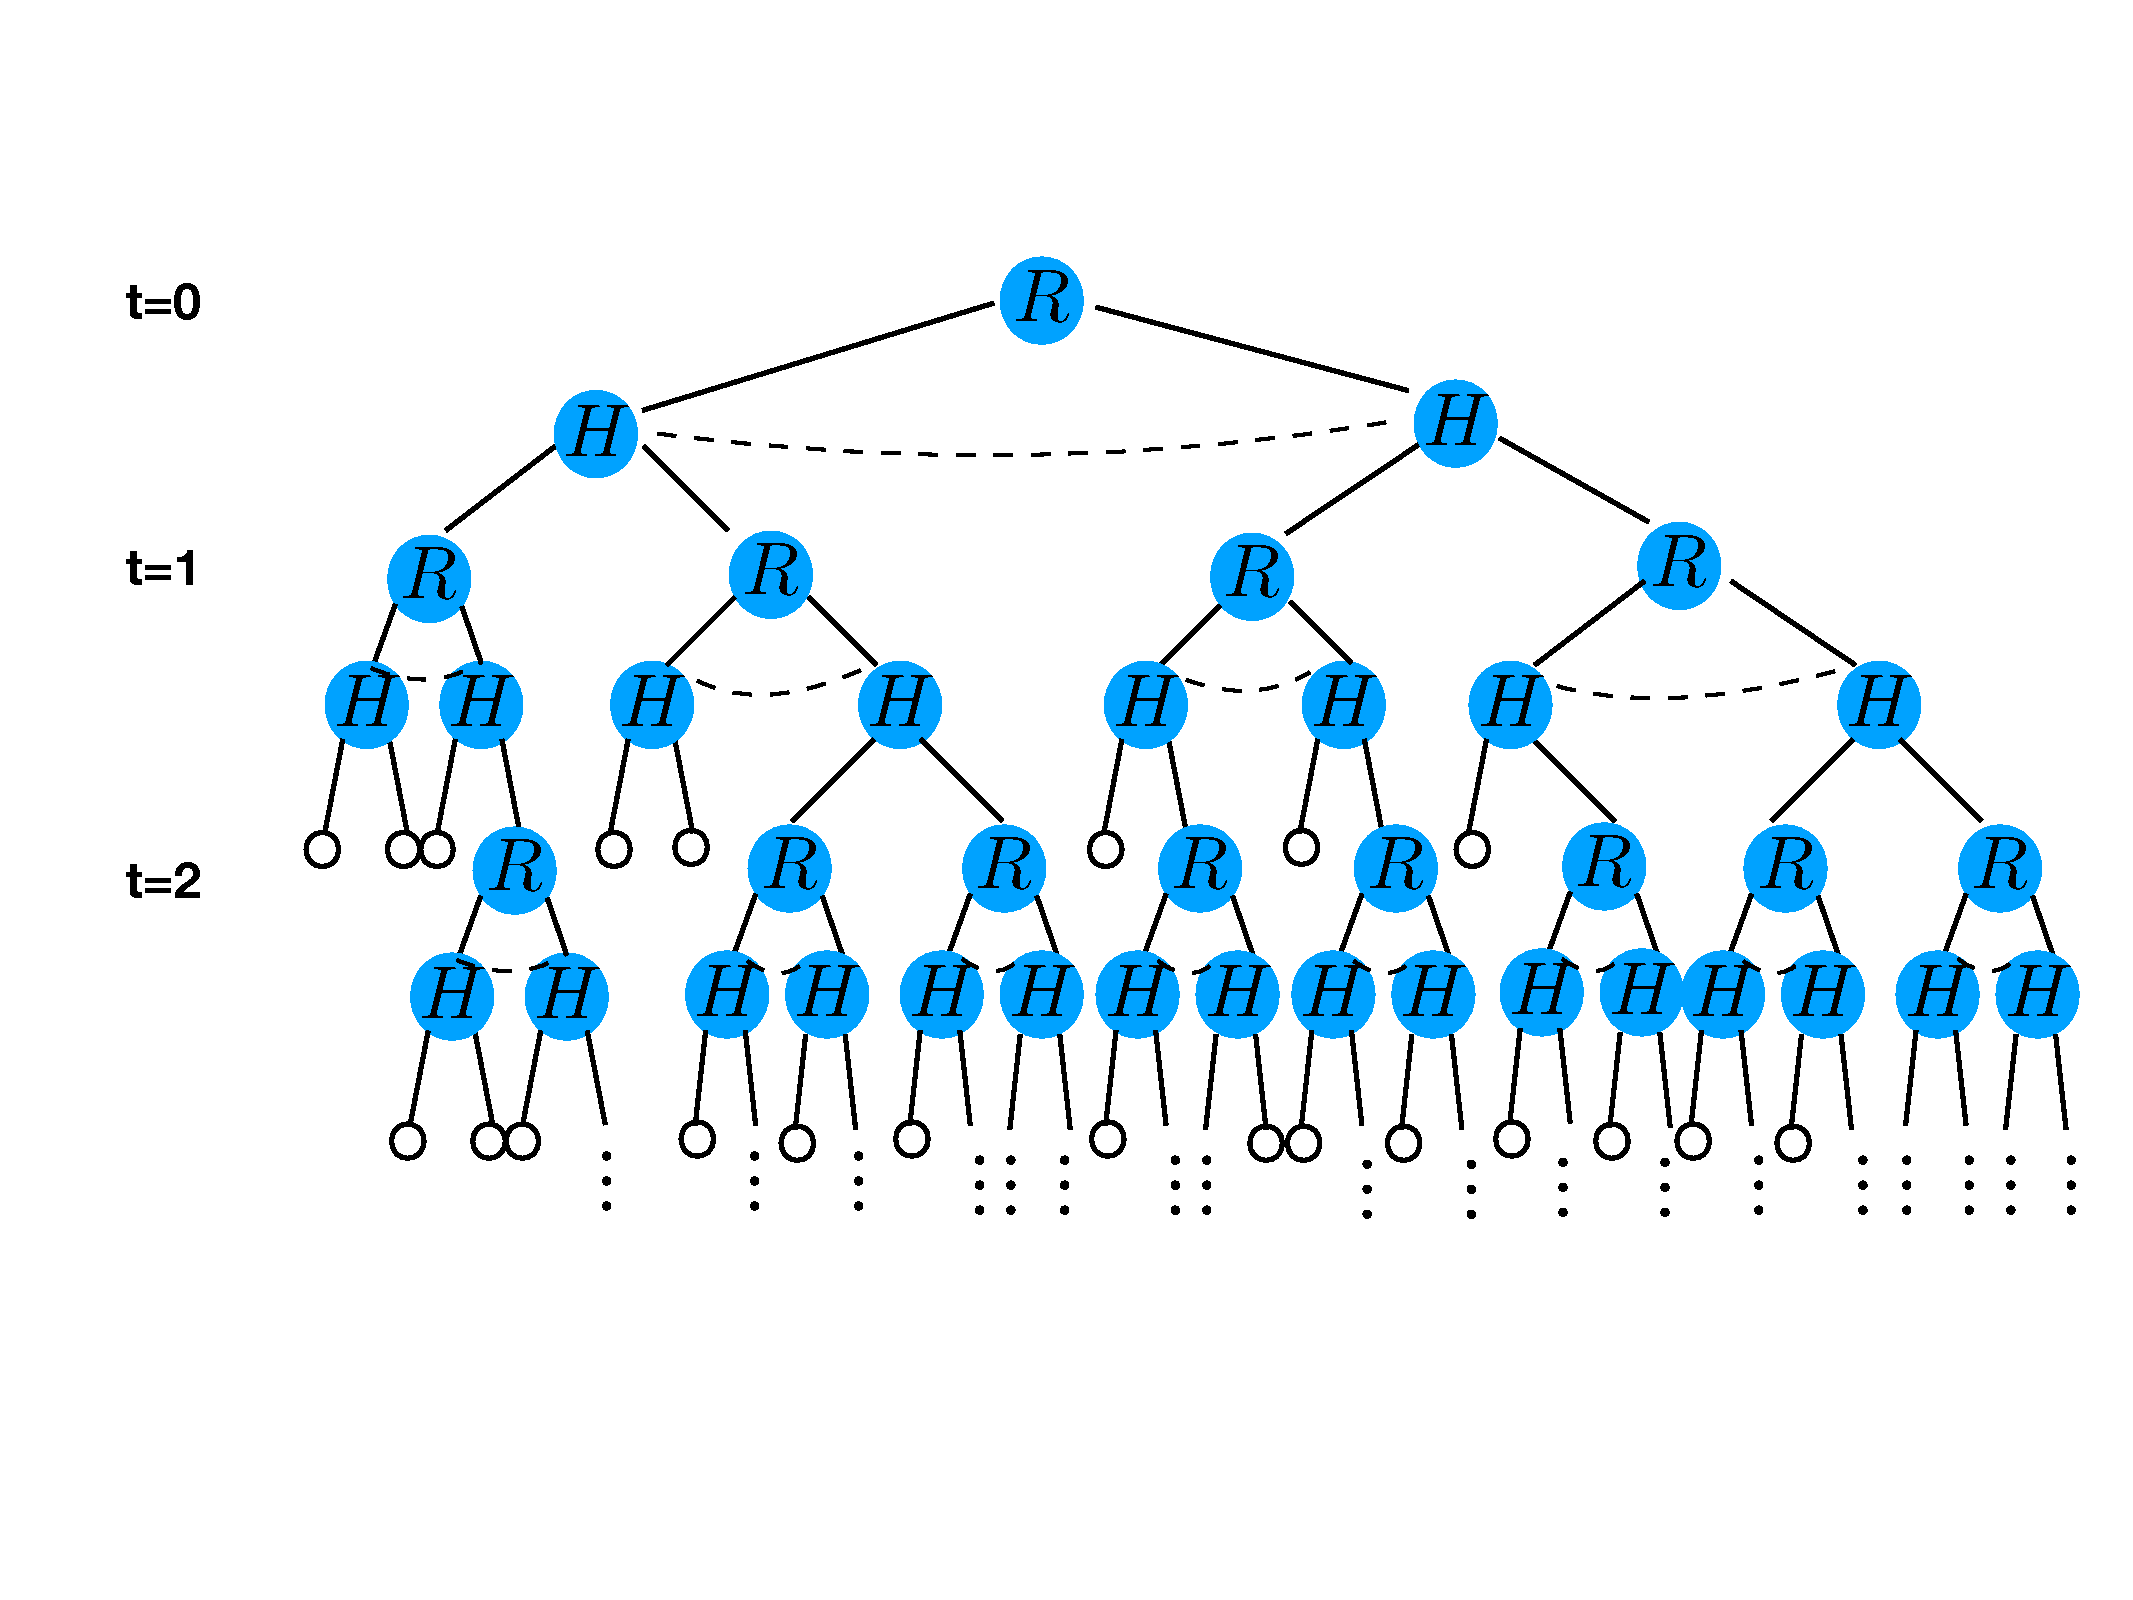
\includegraphics[scale=0.21]{game_tree}
	\vspace{-5em}
	%\hspace{-5em}
	\caption{Two-player human-robot interaction, modeled as a 
		simultaneous-move game. }
	\vspace{-1.4em}
	\label{fig:game_tree}
\end{figure}

\textbf{Action profile prediction, strategy evaluation, and search for 
solution action sequence}:

We note that the policy of how an agent $i$ makes his high-level decision can 
be abbreviated as a function of his (possibly time-variant) type $\theta^i_t$,
\begin{equation}~\label{eq:pi}
a^i_t \sim \pi^i(x_t,\theta^i_t),
\end{equation}
without loss of generality; as $\theta^i_t$ can be time-variant to capture 
human adaptive behaviors in uncertain environments.  

More specifically, at each decision node, agent $i$ chooses action(s) based on 
current state $x_t$ for evaluation. In order to do so, agent $i$ needs to 
compute the following:
\begin{enumerate}
  \item $p(\sigma^{-i}_t|I^i_t,x_t)$: action profile probability of other 
    agents given history set, and
  \item $r^i_t$ or $V^i_T$: 
    reward estimate of current action profile of evaluation, or value estimate 
    if at termination nodes.
\end{enumerate}
%$\theta^i_t$ contains three components: 
%$\theta^i_t = (\theta^i, b^i_t(\theta^{-i}_t),b^i_t(a^{-i}_t))$. 
We note that the form of the game outcomes, either defined by the cumulative 
rewards (as commonly seen in Markov Decision Process) or terminal values (as 
commonly seen in extensive-form games), has no effect on the solution algorithm. 

We also note that, for the purpose of action evaluation, there are other 
suitable computational models, such as that in Equation ~\ref{eq:pi}, 
or the direct mapping from $x^i_t$ to $u^i_t$. Here we 
present this high-level model for its generality, and further implement the 
model to simulate specific human-robot interaction behaviors described in the 
literature, using rules from the behavioral game theory literature.  

Due to the forward state transitions in Markov Games, backward induction, a 
common solution for extensive-form games, is no longer applicable. Instead, 
forward-search approaches such as Monte Carlo Tree Search can be applied: at 
each iteration, randomly sample an action $a^i_t$ for evaluation and then expand the search 
tree by sampling the action profile $p(\sigma^t|I^R_t,x_t)$. To compute the 
reward of a stage game $r^i_t$, or the value at termination nodes $V_T$, 
Equation ~\ref{eq:r_control_input} can be applied by sampling $u_t$ from 
Equation ~\ref{eq:g_function}, given prior on other agents' types 
$p(\theta^{-i}_t)$. 
%players observe past interactions to predict other agents' 
%future policies 
%$\pi^{-i}(x_t,\theta^i_t|\sigma_{0:t-1})$, and to estimate the type parameter 
%$\theta^{-i}_t$ for game outcome estimate $\hat{V}^T(x_T,\sigma_T,\theta_t)$. When new 
%observations come in, both the predictive model on other agents' policies and 
%the type parameter estimate are updated. 

%\vspace{-.2em}
\textbf{Online solutions with prediction model updates}:
%\vspace{-.2em}

When planning for long-horizon purposes, agents ideally want to optimize their 
outcome considering full-horizon reward accumulation, as introduced in Equation 
~\ref{eq:optimal}. However, due to modeling errors and typed behaviors among 
humans, pre-trained models may not well accommodate newly observed behaviors. 
Pre-computed solutions therefore may not suit well to the newly 
encountered agents, therefore, online re-plan is needed to well adapt to new 
situations, using real-time received observation data. 
Inaccurate prediction includes those of other agents' future action profiles, action realizations, and state transitions. 

Therefore we are proposing an \textit{online game 
strategies} as the solution to deal with real-world uncertainties. Instead of running search algorithms to solve for the total 
horizon, the agent will run \textit{belief updates} whenever new 
observations arrive, and \textit{re-plan for certain horizon} from 
current time $t$, for as much lookahead horizon $H$ as computational resource 
allows. We assume agents have knowledge of the termination timing, $\beta_t$, 
even in the dynamic setting.

The following provides a detailed explanation regarding the belief update and 
Receding-horizon planning of each agent.
 
\subsubsection{belief updates}\label{sec:belief_update}
During real-world interactions, observations can be from direct measures, such as the relative positions and velocities of all agents. Observations can also be implicit as to infer private messages, through ways like eye contacts or body languages, to express messages such as intent~\cite{knepper2017implicit}.

With either form of observations, $o^i_{t:t+\tau} \in O^i$, where $1/\tau$ is the 
observation  
update rate and $O^i$ is his observation data space, agents can better infer about 
future motions of the other agents. Given computational models for motion 
predictions, such as $u^{-i}_t \sim g^{-i}(x_t,a^{-i},\theta^{-i}_t)$ proposed 
in our framework (but not restricted to such formulation), to plan in the 
high-level action space $A^i$, agent $i$ needs to update his beliefs of the 
following:

(a) Future strategy profiles of other agents $b^i_t(\sigma^{-i}_{t:T}|x_l,I^i_l)$: 
the strategy profile prediction based on history plays, $p(\sigma_l|x_l,I^i_l)$, 
where $t\leq l\leq T$ is the future time step of 
interest.

(b) Type estimate of other agents $b^i_t(\theta_t^{-i})$: 
the type estimate $p(\theta^{-i}_t|o^i_{t:t-\tau},\theta^{-i}_{t-\tau})$ (in 
the Bayesian setting), in order to sample the joint state transition function 
$\mathcal{T}$ and to compute action reward $r^i_t$.


We note that belief updates are usually computationally cheap, so agents may run it at a high rate (potentially higher than re-plan rate) to deal with noisy 
observations.
 
\subsubsection{Receding-horizon planning}\label{sec:receding}
Due to the potential demand of fast re-planning in dynamic environments, agents may only be computationally available to plan for finite-step lookahead $L<T$. Therefore, at each time step $t=l$,$l<T$, agents instead try to optimize for $t=l:L'$, where $L'=min(l+L,T)$, based on updated model of future strategy 
anticipation of other agents' $p(\sigma_{l:L'}|x_l,I^i_l)$. This online re-planning 
for finite horizon strategy, known as receding-horizon planning, can be formulated as the following:
\begin{equation}
  \begin{aligned}
  a^{i*}_{l:L'} = \argmax_{a^i_{l:L'}} 
  \Sigma_{t=l}^{L'} 
  \mathbb{E}_{x_t,\sigma_{t},\theta_t|\mathcal{T},I^i_t} \big{[}
    r^i(x_t,\sigma_t,&\theta_t)\big{]}+ \\
    \hat{V}^i_{L'+1}(x_L',\sigma_L',&\theta_L'), 
  \end{aligned}
  \end{equation}
where $\hat{V}_{L+1}(x_L,\sigma_L,\theta_L)$ is the cost-to-go estimate for the following $\sigma_L'$ from $t=L'+1$ to $T$.

For coordination games, it is usually true that the earlier the termination, 
the better the final outcome is. One game example is the bargaining game with 
benefit discounts. 
Take another example of the table-turning coordination task, the faster the two agents reach 
agreement on the direction to go, the earlier they start wasting efforts and make progress, despite the 
potentially suboptimal (longer) route selection. Therefore, biased search to 
strategies with early 
termination has its empirically advantage; agents can even trade off 
computation depth with breadth to better explore its action profile. 

\textbf{Strategy response time and turn-taking formulation:}
Since high-level actions or intents are not directly observable by other 
agents, as suggested by Section ~\ref{sec:belief_update}, strategies take time 
for other agents to infer; further, agents need time to replan to newly 
observed strategy, and to execute the new plan with potential changes in 
motions. As a result, with proper waiting time after the initial action, the 
decision timing of both agents can be clearly separated to prevent 
oscillations, which transfers the game formulation into turn-taking, as 
illustrated in Figure ~\ref{fig:turn_taking}. 
Turn-taking games simplify the 
simulation setting by neglecting current time action profile sampling to 
predict other agents' concurrent actions, therefore save computation. 
\begin{figure}[t]
      \centering
      \vspace{-1em}
      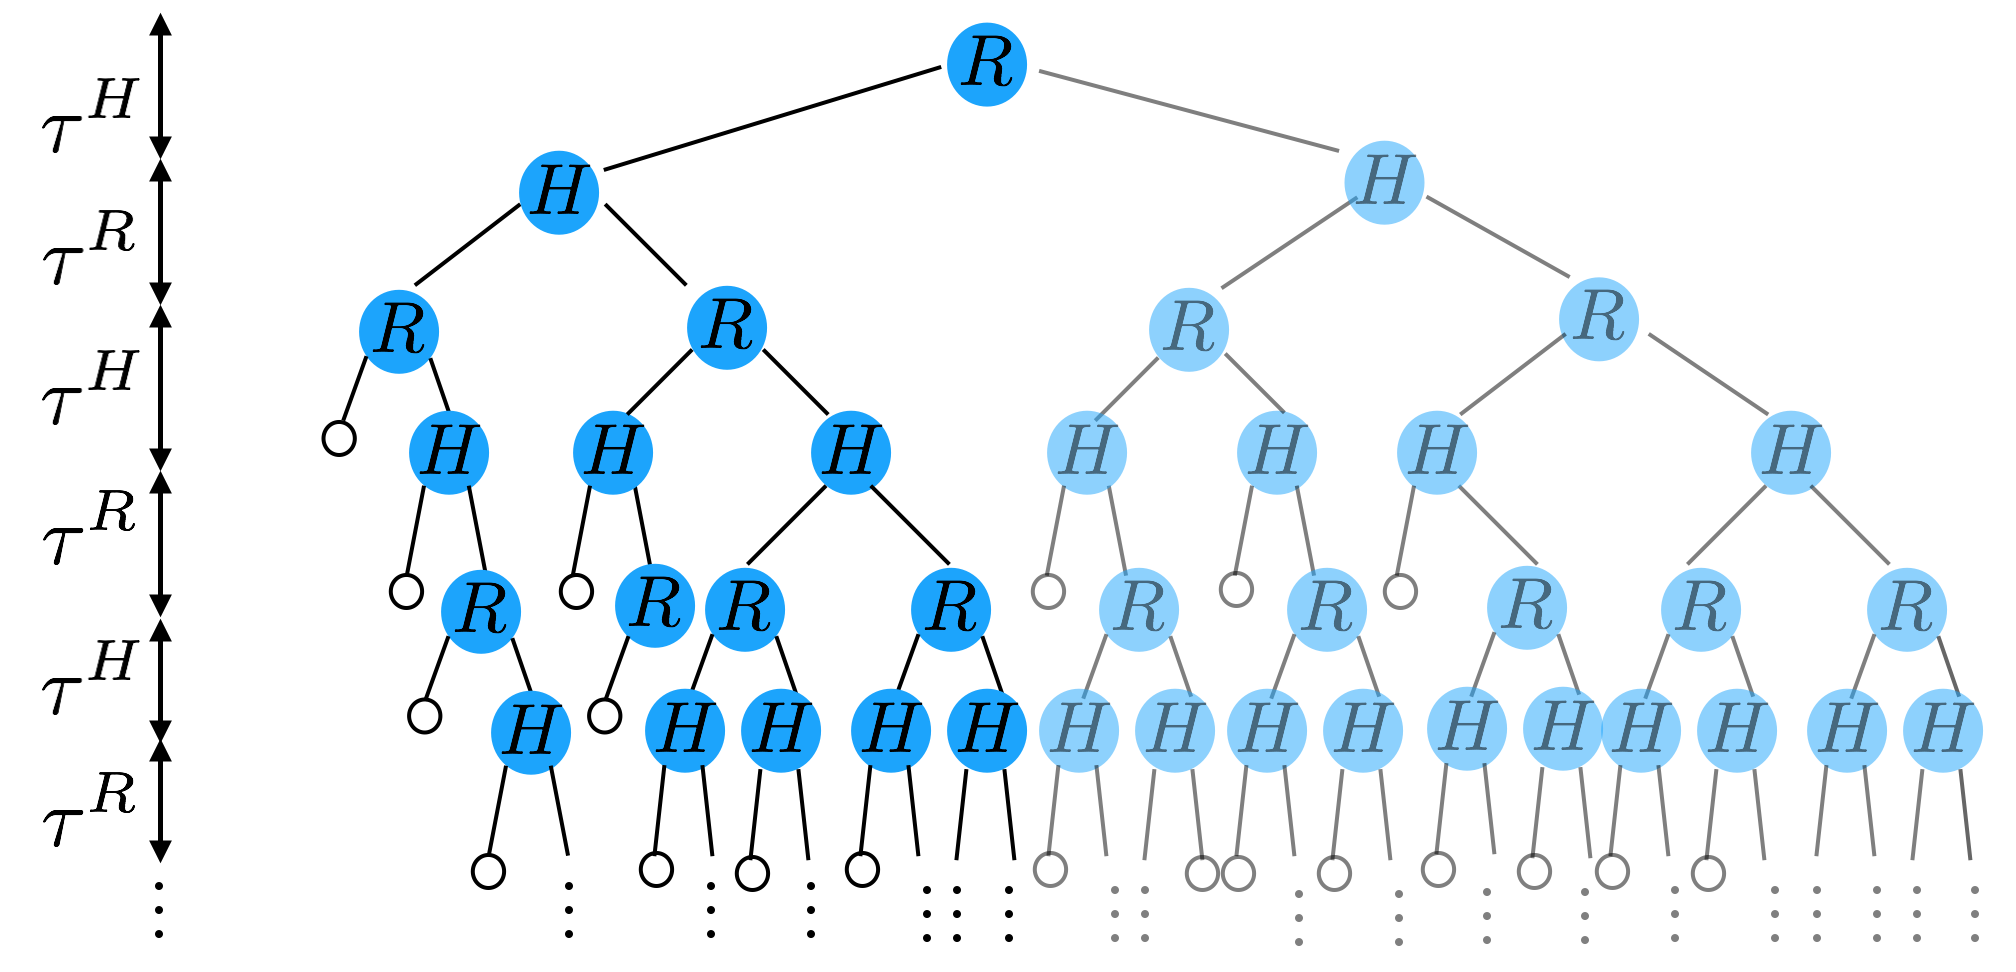
\includegraphics[scale=0.2]{turn_taking}
      \vspace{-1.4em}
      %\hspace{-5em}
      \caption{
        Human-robot turn-taking games with robot anticipating action value based on finite-horizon predictions. $\tau^R$ and $\tau^H$ are approximate time intervals for robot and human response times. The game may terminate at either player's decision nodes.}
      \vspace{-1.7em}
     \label{fig:turn_taking}
\end{figure}
\section{Human Behaviors}\label{sec:human_behavior}
Since one of the main purposes of our proposed framework is to model 
\textit{human} interaction with AI agents, we are now introducing our 
hypotheses regarding human behaviors and their decision-making mechanism; by 
implementing these hypotheses into the suggested framework, we will achieve 
better analysis of how different paradigms in human-robot coordination affect 
the overall game result.
\vspace{-.2em}
\subsection{Adaptation to other agents}\label{sec:adaptability}
\vspace{-.2em}
In interaction, oftentimes humans observe other agents and adapt their 
strategies accordingly ~\cite{nikolaidis2016formalizing,yang2017evaluating}. 
This is because humans update their beliefs of the other agents based on past 
interaction; during then, they acquire samples of others' motion realizations 
and strategies, which directly affect their own action rewards $r^H_t$. 
Therefore, adaptation can be seen as a dynamic strategy to maximize self 
interests. We incorporate such behaviors in our proposed framework 
through the dynamic type parameter $\theta^H_t$, and refer human adaptive 
policy to Equation ~\ref{eq:pi}. 

Further, we propose that a human's type $\theta^H_t$ is parameterized by a 
static parameter $z^H$, and a dynamic inference parameter 
$b^H_t(\theta^{-H}_t)$. The static parameter, $z^H$, is associated with 
domain-specific personal 
preferences, such as urgency to travel to destination, which do not change in 
short period of time; and the 
dynamic inference parameter, $b^H_t(\theta^{-H}_t)$, captures the agent's 
time-evolving \textit{beliefs} of other agents' (potentially dynamic) types. More specifically,
\begin{equation}
  \theta^H_t = \begin{bmatrix}
    z^H \\
    b^H_t(\theta^{-H}_t).
  \end{bmatrix}
\end{equation}

%the static type parameter, $z^H$, features personal preferences such as travel efficiency versus travel energy in navigation domains. The time-variant parameter, $b^H_t(\theta^{-H}_t)$, features humans' perception on other agents' types. 
As for the detailed formulation in human belief, we hypothesize that humans 
possess certain \textit{prior} of the other agents' behaviors, such as assuming 
elderly to move slower and robots to be compliant; when new observations come 
in, humans make use of certain \textit{information budget} to reason about 
other agents' behaviors to update their beliefs.

%Below, we propose our hypothesis on the humans' information budget, which corresponds to their computational capability to infer about other agents' decision-making model. The decision-making model is the policy that outputs the agent's high-level action(s):
\subsection{Depth of Inference and Biased Adaptation}
We now define the concept of \textit{information budget} to be an agent's 
computational capability to infer about other agents' strategy, 
which includes assumptions over their decision-making model. Here, the 
decision-making model is referred to the policy that outputs 
the agent's high-level action(s), i.e., 
$a^i_{t:t+L} \sim \pi^i(x_t,\theta^i_t)$. With different information budgets, 
agents can update their beliefs based on different assumptions over the 
other agents' decision-making model. 
The categories of \textit{information budget} are outlined below:

\begin{itemize}
	\item \textbf{Zero Information} - $b^i_t(\theta^{-i}_t) = \emptyset$. Agents 
    allocate zero budget, therefore keep no information of the other agents' 
    behaviors during interaction; they 
    parametrize their policies solely based on (static) personal preferences, 
    but make 
    no use of other agents' actions/motions to characterize game outcomes. 
    Such agents pay no attention to the game, and we 
    assume \textit{aware} humans do \textit{not} belong to this category.
	\item \textbf{One-Layer Inference} - $b^i_t(\theta^{-i}_t) = \hat{z}^{-i}$. 
    Agents assume the other agents to act only according to their static 
    preferences, $z^{-i}$, which means that they assume others to maintain no 
    information of themselves, $b^i_t(b^{-i}_t(\theta^i_t))=\emptyset$.  
    Therefore, agents adapt to the others as if their own actions have no 
    impact on other agents' strategies or decision-making model, parametrized 
    as 
    $p(a^{-i}_{t:t+L}|x_t, z^{-i})$. We assume humans belong to this 
    category while interacting with robots and will apply it for planning 
    inference in our framework.
	\item \textbf{Two-Layer Inference} - $b^i_t(\theta^{-i}_t) = [\hat{z}^{-i}, \hat{\hat{z}}^i]$. Agents assume the other agents are also adaptive to themselves,
	$\theta^{-i}_t = [z^{-i}, \hat{z}^{i}]$, with one-layer inference. 
    Therefore, when planning for more than one period, agents act adaptively, 
    at the same time evaluating their actions' potential impacts on the 
    other agents' future strategies. For example, when planning for only one game period, 
    agents with the budget to compute two-layer inference plan according to 
    what they 
    predict the others' predictions about themselves 
    $a^i_t \sim \pi^i(x_t, b^i_t(\pi^{-i}(x_t,b^{-i}_t(\pi^i(x_t,{z}^i)))))$
    . When applied for long-horizon planning, agents need to distinguish 
    updates for either $\hat{z}^{-i}$ or $\hat{\hat{z}}^i$, and replan while 
    considering the others' one-layer inference of their own choices of 
    actions. 
    
    Due to the intrinsic complexity, this is the maximal budget we assume 
    humans can afford for real-time inference, and is assumed only 
    affordable for one-shot games but not for long-horizon planning. 
\end{itemize}

Therefore, with the information budget assumption over human inference for long-horizon 
planning, $b^H_t(\theta^H_t) = \hat{z}^{-H}$, we consider human policies 
being adaptive to their perceived, presumably static, behavior of other 
agents. The higher adaptation rate is, the more compliant they 
appear to the other agents' strategies, therefore, more flexible in the joint policy. 

\textit{Biased Adaptation:}

Although $\theta^i_t$ may be partially inferred by other agents $-i$ through 
observations, it is assumed to be not directly observable. 
Type $\theta^H_t$ can be treated as 
the \textit{mental state} on human agents, which are 
hidden from other agents, sometimes, even from themselves.  

The more complex the domain is, the more complicated the way type is related 
to an agent's policy. Given prior estimate of such hidden parameter and its 
belief update rule, sometimes its variables may have coupled effects to the 
resultant observations. In that case, the agent has extra degrees of freedom to 
allocate different levels of attention on 
each variable to apply belief updates, therefore only that the 
agent most concerns gets updated. We refer this as \textit{biased adaptation} in human 
behavior, which saves computation for both belief updates and replanning.  

\textit{Human Lookahead Planning:}
%\color{red}\subsubsection{Bounded memory belief updates}
%***I AM NOT SURE WHY WE ARE TALKING ABOUT THIS***As introduced in Section ~\ref{sec:belief_update}, we also assume humans maintain their 
%beliefs of other agents' types as well as their future strategy profile through out online planning. Here, we further assume humans to either run Bayesian updates, or possess \textit{bounded} memory on past observations and interaction history for belief updates\cite{nikolaidis2016formalizing}: $b^H_t(\sigma_{t}|I^i_{t-(t-n)}),$ and $b^H_t(\theta^{-i}_t|o_{t-n:t})$.

%\subsubsection{Finite-step lookahead}
As introduced in Section ~\ref{sec:receding}, we also assume humans re-plan 
online with finite-step lookahead, $L^H<T$, with belief updates on prediction 
models such as the strategy profile of other agents 
$b^H_t(\pi^{-H}(x_t,\theta^{-H}_t))$. Finite-step lookahead can be either 
\textit{0-step lookahead} (i.e., $L^H=0$), where agents act as if the current 
game is the termination game, or \textit{multi-step lookahead} (i.e., $L^H>0$), 
where agents plan as the game has more than one period. We note that if $L^H>0$, 
adaptive behaviors due to belief updates are expected, given information 
budget assumption: $b^H_t(\theta^{-H}_t)\neq \emptyset$.


%\subsubsection{Anticipation of other agents' policy}
%As pointed out in Section ~\ref{sec:human_behavior}, humans adapt their policies based on their beliefs of other agents' behavior. When planning at time $t$, agents predict other agents' action profile $\sigma_{t:t+H}$ based on past interactions:

%\begin{equation}~\label{eq:human_decision1}
%a^H_t \sim \pi^H(x_t, b^H_t(a^{-H}_{t}|\sigma_{0:t-1})).
%\end{equation}

%To anticipate other agents' actions $a^{-H}_{t}|s_{0:t}$, one may assume 
%their policies are non-adaptive, $a^{-H}_t \sim \pi^{-H(x_t,z^{-H})}$, 
%associated with the one-layer inference. 
%(i.e, two-layers inference for planning). In this paper, we discuss human decisions based on only one-layer inference.
%\color{black}
\subsection{Influential factors in human-robot interaction}
As pointed out in Section ~\ref{sec:human_behavior}, human policies for high-level decisions are parametrized by $\theta^i_t$, which include that person's static type $z^H$ and dynamically perceived types $b^H_t(\theta^{-H}_t)$ of other agents. With different perceptions on the other, humans act differently. For example, pedestrians take over others' roads when they are in a hurry; however, they yield when encountering the elderly. Similar situation 
applies to human-robot interaction: people have distinctive behaviors based on their prior assumptions of robots, which affect their policies and their adaptabilities when new observations come in. In this section we discuss how to use the above proposed model in order to describe	 existing phenomena in human-robot interactions. 

\subsubsection{Perceived robot capability}~\label{sec:perceived}
The gap between true robot capability and human perceived robot capability has shown to deteriorate both joint and individual work efficiency in different task domains ~\cite{dragan2015effects}. Here, we characterize human perceived robot capability for human-robot interaction into two categories which are functional capability and social inference capability.

\begin{itemize}
	\item \textit{Functional capability - } This includes the belief of whether a robot is able to \textit{identify interaction}. Before engaging interactions, agents need to ensure that $\mathcal{C}_{PI}$ and $\mathcal{C}_{MA}$ are met by all parties, or else confusions may arise. Due to lack of social signaling capability, such as gazes, humans may be uncertain whether the robot is aware of the potential interactions. This may result in distantly-avoiding behaviors through out the interaction, since people are not sure whether they should engage ~\cite{dragan2015effects}. This also includes the knowledge of robot action set, $A^R$, and the confidence of whether the robot is able to \textit{succeed in its target actions}, $a^R_t$, especially when complex domains are considered ~\cite{chen2018planning}. 
	\item \textit{Social inference capability - } This involves the question whether human perceive the robot to be capable of engaging with. Implicit communication has a big part in most interactions ~\cite{knepper2017implicit} and therefore it is very important to be able to notice it. Robots should have the ability to \textit{identify humans' intended high-level actions} based on the inference from past observations, and to \textit{express its own intended action} in a clear, context-aware, or, legible manner ~\cite{dragan2013legibility}. Failing to present such capabilities deteriorates human patience and overall efficiency on given tasks ~\cite{cha2015perceived}. 
\end{itemize}

The above two perceived capabilities are prerequisites for humans to engage in the coordination process with robots. In complex domains, those criteria have shown to be challenging ~\cite{knepper2017implicit}, therefore prior experiences on cross-training, teaching, and learning ~\cite{zhang2017plan} may be required to prepare for natural engagement. 

\subsubsection{Static variables, $z^H$}

\begin{itemize}
	\item \textit{Personal preferences:} Since people have different perception and long-time experience in interactions with the environment, they preserve distinctive characteristics in their behaviors that do not change in short period of time. Therefore, when planning considering joint actions, robots should be aware of such types to plan accordingly for agent comfort and overall efficiency ~\cite{gombolay2015coordination}. In our proposed framework, personal preferences contribute to agents' policy realizations, transition functions, and affect the joint performances. Regarding the reward function, they can be characterized as feature weighting $y^i$~\cite{dorsa2017active}:
	\begin{equation}
	r^i = -y^{iT}C, 
	\end{equation}
	
	where $C$ is some vector of cost function. Take social navigation for 
    example, time delay is a domain-specific cost function, and personal 
    urgency level is the associated weight for the cost term.
	\item \textit{Level of self-interest:} When agents are deployed in public environments, the notion of public welfare plays in to assess policy fairness ~\cite{fehr2004social}. While the public welfare is the self-interest in collaborative tasks, in non-cooperative games, agents have incentives to deviate from cooperative behaviors for personal benefits ~\cite{fujiwara2015non}. When individuals plan in a shared workspace with personal objectives to achieve, resource conflicts may occur. 
	While cooperative policies are the most efficient for social welfare, agents may gain more resource allocation when playing selfishly. This notion of fairness can be characterized as weighting on all parties' interest $\alpha^i$:
	\begin{equation}
	r'^{i} = \alpha^ir^i+ \small{\frac{1-\alpha^i}{k-1}}\sum r^{-i}.
	\end{equation}
	
	%\begin{equation}
	%r^{i'} = \alpha^ir^i+ \small{\frac{1-\alpha^i}{k-1}}\sum_{-i} r^{-i}.
	%\end{equation}
\end{itemize}

We note that the level of self-interest, $\alpha^i$, and the personal preferences, $y^i$, jointly contribute to the static preferences, $z^i$.

\subsubsection{Dynamic parameter, $b^H_t(z^{R})$}% and reciprocity}
\begin{itemize}
  \item \textit{Perceived robot preferences:} As humans have domain-specific 
    preferences, they also infer such preferences of the robot to predict 
    their strategy. Take social navigation for example, it could be the 
    perceived level of urgency of the robot given observed tasks at hand.   
  \item \textit{Perceived robot level of self-interest, or, social trust on collaborativity:}
  Perceived capabilities are preliminary for human trust to interact with robots ~\cite{yang2017evaluating}, since the knowledge of the action set of the robot enables 
human prediction of robot future actions. When there are resource conflicts in shared workspaces, self-interested agents may not be socially compliant to the other agents. 
In this case, trust on social collaborativity in conflicted situations, captured by humans' belief of robot static type $b^H_t(z^R)$, affects human policies through their anticipation of robot policy. While perceiving robots as socially trust-worthy agents, humans predict robots to have non-hostile behaviors and may cooperate at ease.   
\end{itemize}



\section{Problem Instantiation}
In this section we instantiate the framework on 2-player human-robot navigation with path 
crossing, shown in Figure ~\ref{fig:intro}.

%\subsection{???Intention-aware social navigation}

Great progress has been made in the past two decades in pedestrian simulations ~\cite{karamouzas2009predictive,zanlungo2011social}, robot navigation with human predictive models ~\cite{trautman2010unfreezing,kuderer2012feature}, and socially-friendly robot planning ~\cite{mavrogiannis2016decentralized,chen2017socially}, to smoothly deploy robots in human workspaces. In human-robot interaction community, robot motion legibility has gained attention for human understanding ~\cite{dragan2013legibility}, and the concept of trajectory interpretability has been applied on robot navigation in crowded environments to identify goals of pedestrians ~\cite{bai2015intention,unhelkar2015human}. 

   \begin{figure}[t]
      \centering
      \vspace{-1em}
      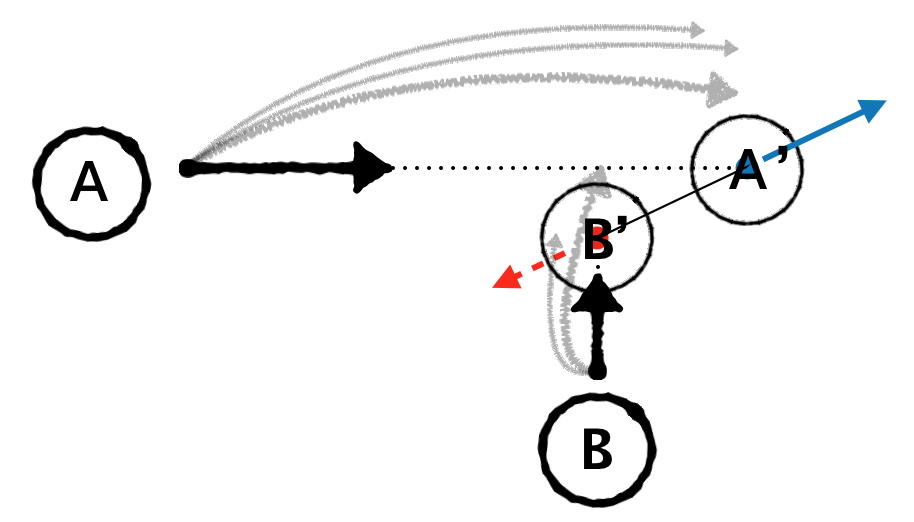
\includegraphics[scale=0.27]{pedestrian_avoidance}
      \vspace{-1em}
      %\hspace{-5em}
      \caption{Collision avoidance actions based on closest position estimate. 
      Red dashed arrow (social force direction): yielding agent with later 
      arrival timing at the intersection; blue solid arrow: passing-first agent. }
      \vspace{-1.5em}
     \label{fig:legibility}
   \end{figure}

In this section we make use of the social force model with explicit collision prediction ~\cite{zanlungo2011social}, which was inspired by the social-force model but equipped with explicit avoidance behaviors. Other choices of human behavioral model for action realizations 
$g(x_t,a^H_t,\theta^H_t)$ can also fit in the framework for simulation; we choose this model for its underlying motion \textit{legibility} concept in distinguishing choices of avoidance behaviors, as can be seen in Figure ~\ref{fig:legibility}.  

When two agents have intersecting paths and have similar timing to arrive at the intersection, explicit avoidance behaviors are involved. Particularly, an agent has to decide whether to avoid in front or behind the other. This leaves the coordination to agree on two action combinations: (passing$\_$first,yielding), or (yielding,passing$\_$first). \textcolor{red}{***shouldn't it be:(passing$\_$first,yielding), or (yielding$\_$first,passing)?***}

We define the state space as following: $x_t^R = \begin{bmatrix}
p^R_t\\
v^R_t
\end{bmatrix}$, and $x_t^H = \begin{bmatrix}
p^H_t\\
v^H_t
\end{bmatrix}$
where $p^R_t, p^H_t$ are the robot's and human's positions, and $v^R_t,v^H_t$ are the robot's and human's velocities, respectively. All variables are described in 2D, therefore, $p^R_t,p^H_t,v^R_t,v^H_t \in \mathbb{R}^2$. 

\subsection{Game start and termination criteria}
As pointed out in Section ~\ref{sec:realtime_game}, to initiate interactive 
behaviors between agents, the potential-interaction criteria $\mathcal{C}_{PI}$ 
and the mutual-awareness criteria $\mathcal{C}_{MA}$ are prerequisites to start the 
game. In path crossing, $\mathcal{C}_{PI}$ is met if:
\begin{enumerate}
  \item two agents have path intersections in near future: 
    $\exists t^H<t^{rH}, t^R<t^{rR}$, such that $v^R_t \times t^R + p^R_t = v^H_t \times t^H +p^H_t$
  \item the arrival timing difference is within certain threshold: $|t^H-t^R|<\delta$
\end{enumerate}
Where $t^{rH}$ is the reaction time (i.e., the time its take to agents to decide to 
engage in the scenario). For pedestrian avoidance, experimental results suggest 
that $t^{rH}$ is on average 4 secs before reaching the intersection ~\cite{pettre2009experiment}. The arrival timing difference depends on agent velocities, the safety margin to keep from other pedestrians, and the noise in estimation. Here, we use an estimate value of $1.5$ sec, which is an upper bound to time difference for which agents respond to the intersecting scenario.

Finally, the game terminates whenever two agents have passed each other, or the minimum relative distance has passed.

\subsection{Intentions in path crossing and time delay}

We will define the agents' action set as following: $A^R = \{a^{pf}, a^y\}$, $A^H = \{a^{pf},a^y\}$, where $a^{pf}$ is corresponding to the class of trajectory realizations of passing first (i.e., in front of the other agent), and $a^y$ is corresponding to the class of yielding to the other. 

Empirical study on human-robot crossing has suggested distinctive velocity and trajectory profiles among two classes of avoidance actions ~\cite{paris2007pedestrian}. Agents who intend to pass first often accelerate and bend their trajectories away from the other. Agents who intend to yield often slow down. Such changes in motion profiles are clear signals for agent passing intents, and one can observe those responses within a short period of time, around $0.7$ sec.


The minimum time for human agents to react to their action changes, $\tau^H$, is assumed to be between $0.7$s to $0.9$s for such a model. For more complex domains, higher values should be considered.

\subsection{Response-time-adapted turn-taking structure}
While the interaction process is modeled as a simultaneous-move game in Section ~\ref{sec:realtime_game}, with the time delays in action realization, it is often played as a \textit{turn-taking} game. 

\begin{figure*}[t]
      \vspace{-1em}
      \centering
      \hspace{-5em}
      \vspace{-1em}
      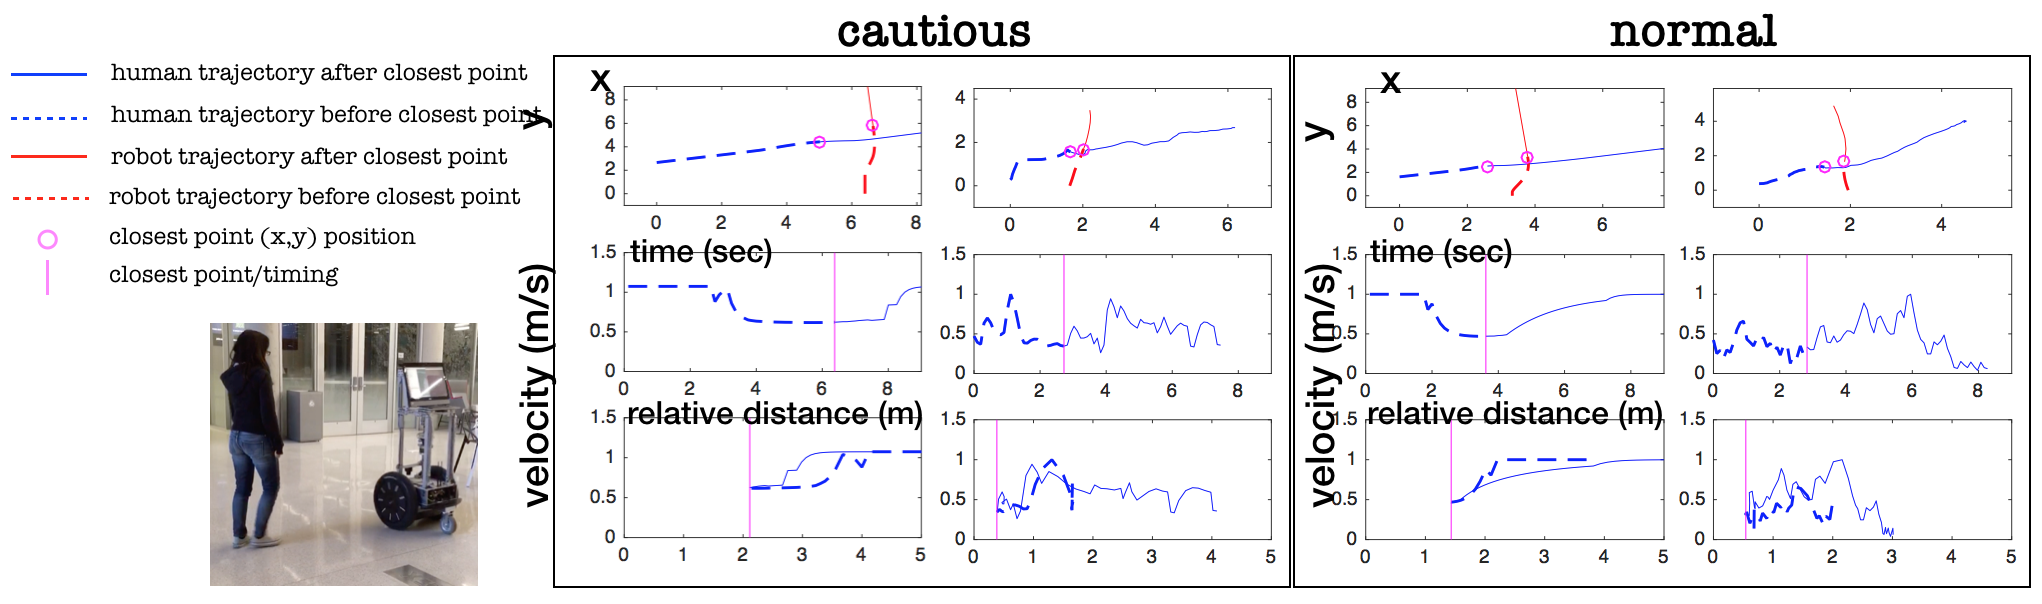
\includegraphics[scale=0.48]{iros_exp}
      \hspace{-5em}
      \caption{SIMULATED pedestrian yielding, compared with REAL recording. We observed many types of behaviors during the experiments, and illustrate one common type in human-robot crossing: cautious, shown in the left box. Compared with people with gradual slow-down and speed-up (noted as ``normal'', shown in the right box), cautious agents wait for the robot until it passes the intersection (shown in the bottom-left photo). We simulate agent yielding and compare the x-y trajectory (top), the velocity profile over time (middle), and relative distance (bottom) with the true recordings, right-side of each box.}
      \vspace{-1.7em}
     \label{fig:cautious_recording}
\end{figure*}

\subsection{Experiments}
We hypothesize that our proposed framework can explain different types of avoidance behaviors when their paths intersect with robots. We use our framework to simulate a particular type, cautious behavior, in comparison with collected trajectory data, to show that the framework can capture distinctive interaction patterns among people. We deploy a mobile robot into a building atrium, and record human crossing trajectories using tracking packages on laser scans ~\cite{leigh2015person}. Eight participants were requested to head towards a set of goals, while the robot followed a given route that intersected with human eight times. The robot was implemented with a local planner with emergent slow-down when sensing an object within $1$ meter. 

\textcolor{red}{***I need you to explain this paragraph to me***} We analyze the results received for 0-step, 1-step, and 2-step lookahead with the same prior on robot strategy profile. With 0-step lookahead, virtual pedestrians act \textcolor{red}{***What does it mean "act compliantly, how?***} compliantly after observing the other agent's action, due to the assumption of immediate termination. With 1-step lookahead, agents assume the game may end with the robot playing minimax strategy, therefore they play based on conservative value estimate. With 2-step lookahead, virtual pedestrians is capable of planning for the optimistic (2nd step) in the worst case robot strategy (1st step). As a result, their behavior in the third case is less conservative compared to the previous two. 

\begin{figure}[t]
      \centering
      \hspace{-5em}
      \vspace{-1.3em}
      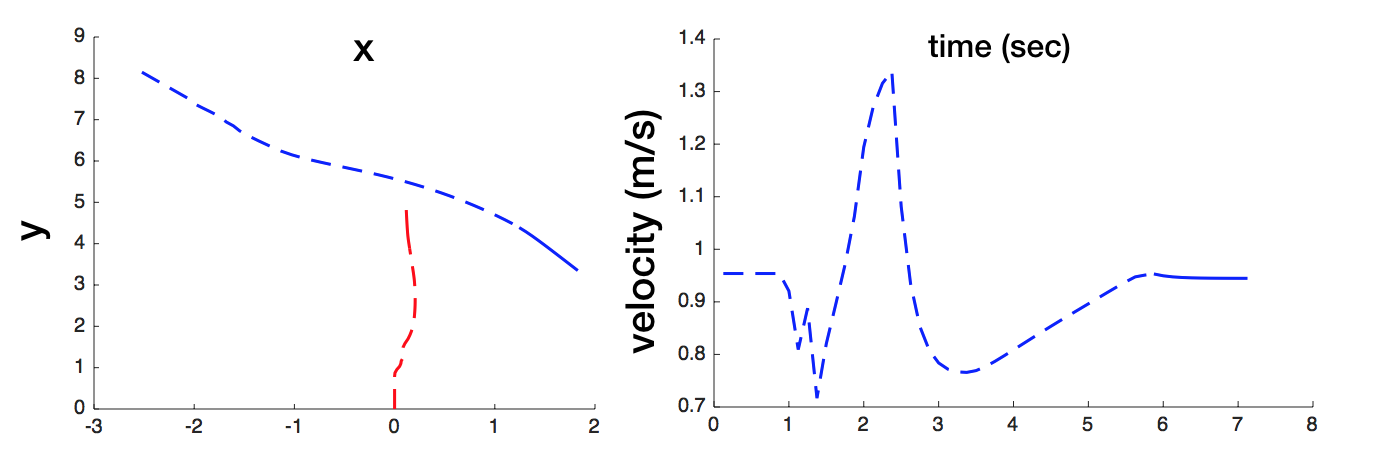
\includegraphics[scale=0.33]{adaptation}
      \hspace{-5em}
      \caption{SIMULATED cautious agent updating belief on robot strategies. While the simulated pedestrian yields at the 
      beginning (with -0.7 sec arrival timing difference), after observing 
      robot yielding behavior, she updates her 
      belief and changes the action in the next time frame.}
      \vspace{-2em}
     \label{fig:adaptation}
\end{figure}

We simulate virtual pedestrians with type $\theta^H_t = [z^H, b^H_t(z^R)]$, 2-step lookahead, memory bound on interaction history = 2, in the turn-taking formulation. This is associated with the decision-making capacity to reason: ``what would the robot do after seeing my action, and what I could do to in reaction to that action?''. Other combinations can be considered. We have the robot choose avoidance actions purely based on arrival timing estimates. It is a simple model for demonstration clarify on human responses; more complex models can be used.

\textcolor{red}{***Comments regarding to Figure \ref{fig:adaptation}: (1) You need to write in the figure what each color stands for. (2) You need to explain (you can do this as a footnote) the different movements in the curves that presents the simulated pedestrian velocity.***}

\subsubsection{Perceived capabilities}
\textcolor{red}{***What are you trying to say in this subsubsection?***} The complete set of perceived capabilities are specified in Section ~\ref{sec:perceived} as 
prerequisites for humans to engage in the coordination process with robots. When dealing with social navigation, people, if noticing robot coming toward them, may be unsure regarding to whether the robot sees them or not (i.e., $\mathcal{C}_{MA}$); whether the robot is aware of the potential collision (i.e., $\mathcal{C}_{PI}$); whether the robot can identify the underlying intention if they choose an avoidance action (i.e., social inference capability on perception); whether they can identify the underlying intention of the robot if it chooses an avoidance action (i.e., social inference capability on motion generation). 

\subsubsection{Types in path crossing}
\textcolor{red}{***I did not understand what are you saying in this paragraph***}Agents perceived other agents' behaviors and update their own type $\theta^H_t$. In social navigation, personal spacing is a common example, as people act repellently more to unfamiliar agents. People's urgency to travel to their own goals are common factors to describe navigation preferences. In simulation, we simulate agents to choose avoidance actions based on the following cost formulation:
\begin{equation}
  r^H_t = -\eta \alpha C^H_t  -(1-\alpha) C^{-H}_t,
\end{equation}
where $C^H_t$ is the estimated time delay, $\eta \in [0,1]$ is the urgency 
level, and $\alpha \in [0,1]$ is the level of self-interest.

\subsubsection{Social trust}
When navigation around a robot, the assumption of whether it is socially compliant affects humans' avoidance decision. We commonly observe, at the beginning of the experiment, participants slow down to wait for the robot to pass first, even when the robot has a later arrival timing; people speed up and stay far from the robot when trying to pass in front, even when the robot is still far from the intersection. 
We refer to this type of behavior as cautious, simulated in Figure ~\ref{fig:cautious_recording} through 
varying the perceived robot level of self-interest: $b^H_t(z^R)$. 

\textcolor{red}{***Comments regarding to Figure \ref{fig:cautious_recording}: (1) It is not clear which squares present the results of the recording and which squares  present the results of the simulation. You should write it next to each relevant column. (2) The axis' titles are not well presented, it looks very messy. I suggest spacing the figure a little bit, so you will have space for the titles. (3) I can not see what is the difference between the cautious and normal agents in the top graphs, it look the same to me. Do you have other recording/simulation in which the normal agent crosses first? Then there will be a difference between the two kinds of agents. (4) Can you add to the figure a map of the routes used in the experiment? I think it will help better understanding of the result and even the experiment itself.*** }

\subsubsection{Human exploration and adaptation}
In the above described experiments we observed many conservative decisions made by human regarding to their crossing (e.g., pedestrians constantly yield to the robot). One agent actually tried passing in front of the robot for a couple of times and then decided to pass first. We consider this process as gradually gaining social trust on the robot; the agent updated her belief of the robot behavior and then adapted her own strategy. Similar behavior was simulated on virtual human with high belief update rate, shown in Figure ~\ref{fig:adaptation}.   

\section{Conclusion and Future Work}
We propose a Markov Game model with time-variant types to analyze human-robot coordination outcome, and propose a human decision-making model to describe phenomena in human-robot interactions. With the framework, we simulate virtual pedestrians with cautious type behaviors on human-robot crossing and compare the results with real-world recording. We also simulate adaptive human behaviors through belief updates on robot policy. In future work, we will further investigate human adaptability criteria based on different prior assumptions on robot behaviors and game convergence given false human assumptions.
%%%%%%%%%%%%%%%%%%%%%%%%%%%%%%%%%%%%%%%%%%%%%%%%%%%%%%%%%%%%%%%%%%%%%%%%%%%%%%%%
\vspace{-0.2em}
\bibliographystyle{plain}
\bibliography{reference}
\end{document}
